\documentclass[twocolumn]{aa}

\usepackage{graphicx}
\usepackage{amsmath,amsfonts,amssymb}
\usepackage{txfonts}
\usepackage{color}
%\usepackage{fixltx2e}
\usepackage{natbib}
%\usepackage{caption,subcaption}
%\usepackage{epsfig}
\usepackage{float}
%\usepackage{stfloats}
\usepackage{dblfloatfix}
\usepackage{afterpage}
\usepackage{ifthen}
\usepackage[morefloats=12]{morefloats}
\usepackage{placeins}
\usepackage{multicol}
\usepackage{makecell}
\usepackage{multirow}
%\usepackage[breaklinks,colorlinks,citecolor=blue]{hyperref}
\bibpunct{(}{)}{;}{a}{}{,}
\usepackage[switch]{lineno}
\definecolor{linkcolor}{rgb}{0.6,0,0}
\definecolor{citecolor}{rgb}{0,0,0.75}
\definecolor{urlcolor}{rgb}{0.12,0.46,0.7}
\usepackage[breaklinks, colorlinks, urlcolor=urlcolor,
    linkcolor=linkcolor,citecolor=citecolor,pdfencoding=auto]{hyperref}
\hypersetup{linktocpage}


%Planck style file, to be used with A&A style to produce Planck papers for publication.
%
% version 28 September 2010 --- useful macros --- CRL
% version 17 October 2010   --- first cut at important instrument values, from Daniele Mennella and
%                               Francois Bouchet, 13 October 2010 --- CRL
% version 18 October 2010   --- LFI FWHM changed to one value per feed, rather than M & S separately
%                               LFI FWHM uncertainties added for individual feeds.  Corrections made
%                               to LFI values. --- Andrea Zacchei
% version 24 October 2010   --- added to and corrected definitions.  No changes made to instrument
%                               quantities. --- CRL 
% version 31 October 2010   --- added definition of \muKHz. --- CRL
%
% version 15 November 2010  --- fixed conflict with aa.cls in definition of \endtable
%                               by naming the command below "\endPlancktable".  See section
%                               13.16 of the Style Guide.
%
% version 06 December 2010  --- Set up names with and without units.
%                               Add \allearlypapers command to ensure that all early papers are
%                               included in the reference list.
%                               Define macro for the name of the 4He JT cooler.
%
% version 07 December 2010  --- removed extraneous "planck2011-1.2" entry in \allearlypapers
%
% version 12 December 2010  --- added \endPlancktablewide command to set tablenotes to the full
%                               page width in the \begin{table*}...\end{table*} environment when
%                               the ``twocolumn'' option is specified in the \documentclass command.
%                               (It would be more elegant to extract the appropriate width from the
%                               aa.cls system at the time of execution, but that is buried more
%                               deeply in the system than I investigated.)
%
% version 05 January 2011   --- added unit \MJysr.  HFI performance values updated per FRB email
%                               01/05/2011 02:38-0800, and Brendan Crill email 01/05/2011 18:08 -0800.
%
% version 06 January 2011   --- changed \scriptscriptstyle primes to \scriptstyle, to better match the
%                               tx fonts used by A&A.
%
% version 07 January 2011   --- modified \allearlypapers to correspond with final early paper list.  
%                               Fixed 545 GHz center frequency.
%
% version 07 January 2011b  --- changed LFI white-noise sensitivity numbers to correct problem with units
%
% version 05 July 2011      --- added \Msol and \Lsol to get the symbols for solar mass and luminosity.
%                               Deleted previous definitions of \solar and \sol, which were equivalent
%                               to the new \Msol.
%
% version 16 August 2011    --- changed comments on \endPlancktable and \endPlancktablewide for clarity
%
% version 11 September 2011 --- changed definition of \tablenote to make footnote labels italic, as per A\&A
%
% version 26 April 2011     --- changed definition of \Planck to agree with what is said in the Style Guide (!)
%
% version 04 Dec 2013       --- included 2013 results references
%
% version 17 Jan 2014       --- included fix to bibtex file v4.3, i.e. \providecommand{\sorthelp}[1]{}
%
% version 26 Jul 2014       --- fixed incompatibility problem with aa.cls v8.0 and v8.2.  v8.2 should now be used
%                               for all Planck papers.
%                           --- fixed problem in definition of "\all2013resultspapers" that introduced a blanck
%                               into the reference to p06b.
%                           --- removed all the parameter definition stuff at the end.  We weren't using it, and
%                               it took up a lot of space.
%
% version 28 Jan 2015       --- added "\alltwentyfiftennresultspapers" and corrected "\all2013resultspapers" to
%                               "\all20thirteenresultspapers",
%
% Usage:  after the \documentclass[traditabstract]{aa} command in the La\TeX\ input file,
%         add this command:      \input Planck.tex


\def\setsymbol#1#2{\expandafter\def\csname #1\endcsname{#2}}
\def\getsymbol#1{\csname #1\endcsname}

%-----------------------------------------------------------------------
% Planck
%-----------------------------------------------------------------------
\def\Planck{\textit{Planck}}

%-----------------------------------------------------------------------
% The Planck Helium-4 JT cooler
%-----------------------------------------------------------------------
\def\HeJT{$^4$He-JT}

%-----------------------------------------------------------------------
% To include all Planck Early Results papers in the reference lists
%-----------------------------------------------------------------------
\def\allearlypapers{\nocite{planck2011-1.1, planck2011-1.3, planck2011-1.4, planck2011-1.5, planck2011-1.6, planck2011-1.7, planck2011-1.10, planck2011-1.10sup, planck2011-5.1a, planck2011-5.1b, planck2011-5.2a, planck2011-5.2b, planck2011-5.2c, planck2011-6.1, planck2011-6.2, planck2011-6.3a, planck2011-6.4a, planck2011-6.4b, planck2011-6.6, planck2011-7.0, planck2011-7.2, planck2011-7.3, planck2011-7.7a, planck2011-7.7b, planck2011-7.12, planck2011-7.13}}

%-----------------------------------------------------------------------
% To include all Planck 2013 Results papers in the reference lists
%-----------------------------------------------------------------------
\def\alltwentythirteenresultspapers{\nocite{planck2013-p01, planck2013-p02, planck2013-p02a, planck2013-p02d, planck2013-p02b, planck2013-p03, planck2013-p03c, planck2013-p03f, planck2013-p03d, planck2013-p03e, planck2013-p01a, planck2013-p06, planck2013-p03a, planck2013-pip88, planck2013-p08, planck2013-p11, planck2013-p12, planck2013-p13, planck2013-p14, planck2013-p15, planck2013-p05b, planck2013-p17, planck2013-p09, planck2013-p09a, planck2013-p20, planck2013-p19, planck2013-pipaberration, planck2013-p05, planck2013-p05a, planck2013-pip56, planck2013-p06b, planck2013-p01a}}

%-----------------------------------------------------------------------
% To include all Planck 2015 Results papers in the reference lists
%-----------------------------------------------------------------------
\def\alltwentyfifteenresultspapers{\nocite{planck2014-a01, planck2014-a03, planck2014-a04, planck2014-a05, planck2014-a06, planck2014-a07, planck2014-a08, planck2014-a09, planck2014-a11, planck2014-a12, planck2014-a13, planck2014-a14, planck2014-a15, planck2014-a16, planck2014-a17, planck2014-a18, planck2014-a19, planck2014-a20, planck2014-a22, planck2014-a24, planck2014-a26, planck2014-a28, planck2014-a29, planck2014-a30, planck2014-a31, planck2014-a35, planck2014-a36, planck2014-a37, planck2014-ES}}

%-----------------------------------------------------------------------
% Tables
%-----------------------------------------------------------------------
\newbox\tablebox    \newdimen\tablewidth
\def\leaderfil{\leaders\hbox to 5pt{\hss.\hss}\hfil}
%
% use the following definition of \endPlancktable for ApJ style notes to tables, set to the 
%         width of the table
% \def\endPlancktable{\tablewidth=\wd\tablebox 
%
% use the following definitions of \endPlancktable and \endPlancktablewide for A&A style notes 
% set to one-column  or full-page width, respectively
\def\endPlancktable{\tablewidth=\columnwidth 
    $$\hss\copy\tablebox\hss$$
    \vskip-\lastskip\vskip -2pt}
\def\endPlancktablewide{\tablewidth=\textwidth 
    $$\hss\copy\tablebox\hss$$
    \vskip-\lastskip\vskip -2pt}
\def\tablenote#1 #2\par{\begingroup \parindent=0.8em
    \abovedisplayshortskip=0pt\belowdisplayshortskip=0pt
    \noindent
    $$\hss\vbox{\hsize\tablewidth \hangindent=\parindent \hangafter=1 \noindent
    \hbox to \parindent{$^#1$\hss}\strut#2\strut\par}\hss$$
    \endgroup}
\def\doubleline{\vskip 3pt\hrule \vskip 1.5pt \hrule \vskip 5pt}

%-----------------------------------------------------------------------
% useful macros
%-----------------------------------------------------------------------
%
\def\L2{\ifmmode L_2\else $L_2$\fi}
%
\def\dtt{\Delta T/T}
\def\DeltaT{\ifmmode \Delta T\else $\Delta T$\fi}
\def\deltat{\ifmmode \Delta t\else $\Delta t$\fi}
\def\fknee{\ifmmode f_{\rm knee}\else $f_{\rm knee}$\fi}
\def\Fmax{\ifmmode F_{\rm max}\else $F_{\rm max}$\fi}
%
\def\solar{\ifmmode{\rm M}_{\mathord\odot}\else${\rm M}_{\mathord\odot}$\fi}
\def\Msolar{\ifmmode{\rm M}_{\mathord\odot}\else${\rm M}_{\mathord\odot}$\fi}
\def\Lsolar{\ifmmode{\rm L}_{\mathord\odot}\else${\rm L}_{\mathord\odot}$\fi}
%
\def\inv{\ifmmode^{-1}\else$^{-1}$\fi}
\def\mo{\ifmmode^{-1}\else$^{-1}$\fi}
\def\sup#1{\ifmmode ^{\rm #1}\else $^{\rm #1}$\fi}
\def\expo#1{\ifmmode \times 10^{#1}\else $\times 10^{#1}$\fi}
%
\def\,{\thinspace}
\def\lsim{\mathrel{\raise .4ex\hbox{\rlap{$<$}\lower 1.2ex\hbox{$\sim$}}}}
\def\gsim{\mathrel{\raise .4ex\hbox{\rlap{$>$}\lower 1.2ex\hbox{$\sim$}}}}
\let\lea=\lsim
\let\gea=\gsim
\def\simprop{\mathrel{\raise .4ex\hbox{\rlap{$\propto$}\lower 1.2ex\hbox{$\sim$}}}}
%
\def\deg{\ifmmode^\circ\else$^\circ$\fi}
\def\pdeg{\ifmmode $\setbox0=\hbox{$^{\circ}$}\rlap{\hskip.11\wd0 .}$^{\circ}
          \else \setbox0=\hbox{$^{\circ}$}\rlap{\hskip.11\wd0 .}$^{\circ}$\fi}
\def\arcs{\ifmmode {^{\scriptstyle\prime\prime}}
          \else $^{\scriptstyle\prime\prime}$\fi}
\def\arcm{\ifmmode {^{\scriptstyle\prime}}
          \else $^{\scriptstyle\prime}$\fi}
\newdimen\sa  \newdimen\sb
\def\parcs{\sa=.07em \sb=.03em
     \ifmmode \hbox{\rlap{.}}^{\scriptstyle\prime\kern -\sb\prime}\hbox{\kern -\sa}
     \else \rlap{.}$^{\scriptstyle\prime\kern -\sb\prime}$\kern -\sa\fi}
\def\parcm{\sa=.08em \sb=.03em
     \ifmmode \hbox{\rlap{.}\kern\sa}^{\scriptstyle\prime}\hbox{\kern-\sb}
     \else \rlap{.}\kern\sa$^{\scriptstyle\prime}$\kern-\sb\fi}
%
\def\ra[#1 #2 #3.#4]{#1\sup{h}#2\sup{m}#3\sup{s}\llap.#4}
\def\dec[#1 #2 #3.#4]{#1\deg#2\arcm#3\arcs\llap.#4}
\def\deco[#1 #2 #3]{#1\deg#2\arcm#3\arcs}
\def\rra[#1 #2]{#1\sup{h}#2\sup{m}}
%
\def\page{\vfill\eject}
\def\dots{\relax\ifmmode \ldots\else $\ldots$\fi}
%
%-----------------------------------------------------------------------
% units
%-----------------------------------------------------------------------
%
\def\WHzsr{\ifmmode $W\,Hz\mo\,sr\mo$\else W\,Hz\mo\,sr\mo\fi}
\def\mHz{\ifmmode $\,mHz$\else \,mHz\fi}
\def\GHz{\ifmmode $\,GHz$\else \,GHz\fi}
\def\mKs{\ifmmode $\,mK\,s$^{1/2}\else \,mK\,s$^{1/2}$\fi}
\def\muKs{\ifmmode \,\mu$K\,s$^{1/2}\else \,$\mu$K\,s$^{1/2}$\fi}
\def\muKRJs{\ifmmode \,\mu$K$_{\rm RJ}$\,s$^{1/2}\else \,$\mu$K$_{\rm RJ}$\,s$^{1/2}$\fi}
\def\muKHz{\ifmmode \,\mu$K\,Hz$^{-1/2}\else \,$\mu$K\,Hz$^{-1/2}$\fi}
\def\MJysr{\ifmmode \,$MJy\,sr\mo$\else \,MJy\,sr\mo\fi}
\def\MJysrmK{\ifmmode \,$MJy\,sr\mo$\,mK$_{\rm CMB}\mo\else \,MJy\,sr\mo\,mK$_{\rm CMB}\mo$\fi}
\def\microns{\ifmmode \,\mu$m$\else \,$\mu$m\fi}
\def\micron{\microns}
\def\muK{\ifmmode \,\mu$K$\else \,$\mu$\hbox{K}\fi}
\def\microK{\ifmmode \,\mu$K$\else \,$\mu$\hbox{K}\fi}
\def\muW{\ifmmode \,\mu$W$\else \,$\mu$\hbox{W}\fi}
\def\kms{\ifmmode $\,km\,s$^{-1}\else \,km\,s$^{-1}$\fi}
\def\kmsMpc{\ifmmode $\,\kms\,Mpc\mo$\else \,\kms\,Mpc\mo\fi}
%
%
%----------------------------------------------------------------------
% set up machinery to list Planck papers in roman numeral order.
%----------------------------------------------------------------------

\providecommand{\sorthelp}[1]{}

\def\WMAP{WMAP}
\def\COBE{COBE}
\def\LCDM{$\Lambda$CDM}
\def\ffp{FFP6}
\def\unionmask{U73}
\def\nside{N_{\mathrm{side}}}

\def\healpix{\texttt{HEALPix}}
\def\commander{\texttt{Commander}}
\def\commanderone{\texttt{Commander1}}
\def\commandertwo{\texttt{Commander2}}
\def\ruler{\texttt{Ruler}}
\def\comrul{\texttt{Commander-Ruler}}
\def\CR{\texttt{C-R}}
\def\nilc{\texttt{NILC}}
\def\gnilc{\texttt{GNILC}}
\def\sevem{\texttt{SEVEM}}
\def\smica{\texttt{SMICA}}
\def\CamSpec{\texttt{CamSpec}}
\def\Plik{\texttt{Plik}}
\def\XFaster{\texttt{XFaster}}

\renewcommand{\d}[0]{\vec{d}}
\renewcommand{\t}[0]{\vec{t}}
\newcommand{\A}[0]{\tens{A}}
%\newcommand{\Y}[0]{\tens{Y}}
\newcommand{\Y}[0]{\tens{Y}}
\newcommand{\n}[0]{\vec{n}}
\newcommand{\red}[0]{\color{red}}
\newcommand{\green}[0]{\color{green}}
\newcommand{\s}[0]{\vec{s}}
\renewcommand{\a}[0]{\vec{a}}
\newcommand{\m}[0]{\vec{m}}
\newcommand{\f}[0]{\vec{f}}
\newcommand{\F}[0]{\tens{F}}
\newcommand{\B}[0]{\tens{B}}
\newcommand{\T}[0]{\tens{T}}
\newcommand{\Cp}[0]{\tens{C}}
\renewcommand{\L}[0]{\tens{L}}
\newcommand{\g}[0]{\vec{g}}
\newcommand{\N}[0]{\tens{N}}
\newcommand{\M}[0]{\tens{M}}
\newcommand{\iN}[0]{\tens{N}^{-1}}
\newcommand{\iM}[0]{\tens{M}^{-1}}
\newcommand{\w}[0]{\vec{w}}
\renewcommand{\S}[0]{\tens{S}}
\renewcommand{\r}[0]{\vec{r}}
\renewcommand{\u}[0]{\vec{u}}
\newcommand{\q}[0]{\vec{q}}
\renewcommand{\v}[0]{\vec{v}}
\renewcommand{\P}[0]{\tens{P}}
\newcommand{\dt}[0]{d_t}
\newcommand{\di}[0]{d_i}
\newcommand{\nt}[0]{n_t}
\newcommand{\st}[0]{s_t}
\newcommand{\mt}[0]{m_t}
\newcommand{\ft}[0]{f_t}
\newcommand{\Te}[0]{T_{\rm e}}
\newcommand{\EM}[0]{\rm EM}
\newcommand{\mathsc}[1]{{\normalfont\textsc{#1}}}
\newcommand{\hi}{\ensuremath{\mathsc {Hi}}}


\newcommand{\BP}{\textsc{BeyondPlanck}}

\def\bC{\tens{C}}
\def\ba{\vec{a}}
\def\ncha{N_\mathrm{cha}}
\def\nfg{N_\mathrm{fg}}

%\modulolinenumbers[5]
%\linenumbers

\newcommand{\includegraphicsdpi}[3]{
    \pdfimageresolution=#1  % Change the dpi of images
    \includegraphics[#2]{#3}
    \pdfimageresolution=72  % Change it back to the default
}

\renewcommand{\topfraction}{1.0}	% max fraction of floats at top
    \renewcommand{\bottomfraction}{1.0}	% max fraction of floats at bottom
    %   Parameters for TEXT pages (not float pages):
    \setcounter{topnumber}{2}
    \setcounter{bottomnumber}{2}
    \setcounter{totalnumber}{4}     % 2 may work better
    \setcounter{dbltopnumber}{2}    % for 2-column pages
    \renewcommand{\dbltopfraction}{0.9}	% fit big float above 2-col. text
    \renewcommand{\textfraction}{0.04}	% allow minimal text w. figs
    %   Parameters for FLOAT pages (not text pages):
    \renewcommand{\floatpagefraction}{0.9}	% require fuller float pages
	% N.B.: floatpagefraction MUST be less than topfraction !!
    \renewcommand{\dblfloatpagefraction}{0.9}	% require fuller float pages

\def\adj{^{\dagger}}
\def\tp{^{\rm T}}
\def\inv{^{-1}}
\def\lm{{\ell m}}

\begin{document}

\title{\textit{BeyondPlanck} results. 19. Low-Level Processing}
%This author list corresponds to \title{Author list for L04\_CMB\_Foregrounds\_Extraction}
%Prepared by M. Lopez-Caniego (Marcos.Lopez.Caniego@sciops.esa.int), ESAC/ESA
%This version is from Thu Jul 12 18:11:48 2018 CET
%\subtitle{There are 152 co-authors in this list}
\newcommand{\nersc}[0]{1}
\newcommand{\princeton}[0]{2}
\newcommand{\helsinkiA}[0]{3}
\newcommand{\milanoA}[0]{4}
\newcommand{\triesteA}[0]{5}
\newcommand{\haverford}[0]{6}
\newcommand{\helsinkiB}[0]{7}
\newcommand{\triesteB}[0]{8}
\newcommand{\milanoB}[0]{9}
\newcommand{\milanoC}[0]{10}
\newcommand{\oslo}[0]{11}
\newcommand{\jpl}[0]{12}
\newcommand{\mpa}[0]{13}
\newcommand{\planetek}[0]{14}
\author{\small
M.~Galloway\inst{\oslo}\thanks{Corresponding author: M.~Galloway; \url{mathew.galloway@astro.uio.no}}
\and
\textcolor{black}{D.~Herman}\inst{\oslo}
\and
K.~J.~Andersen\inst{\oslo}
\and
\textcolor{black}{R.~Aurlien}\inst{\oslo}
\and
\textcolor{black}{R.~Banerji}\inst{\oslo}
\and
M.~Bersanelli\inst{\milanoA, \milanoB, \milanoC}
\and
S.~Bertocco\inst{\triesteB}
\and
M.~Brilenkov\inst{\oslo}
\and
M.~Carbone\inst{\planetek}
\and
L.~P.~L.~Colombo\inst{\milanoA}
\and
H.~K.~Eriksen\inst{\oslo}
\and
J.~R.~Eskilt\inst{\oslo}
\and
\textcolor{black}{M.~K.~Foss}\inst{\oslo}
\and
C.~Franceschet\inst{\milanoA,\milanoC}
\and
\textcolor{black}{U.~Fuskeland}\inst{\oslo}
\and
S.~Galeotta\inst{\triesteB}
\and
M.~Galloway\inst{\oslo}
\and
S.~Gerakakis\inst{\planetek}
\and
E.~Gjerl{\o}w\inst{\oslo}
\and
\textcolor{black}{B.~Hensley}\inst{\princeton}
\and
M.~Iacobellis\inst{\planetek}
\and
M.~Ieronymaki\inst{\planetek}
\and
\textcolor{black}{H.~T.~Ihle}\inst{\oslo}
\and
J.~B.~Jewell\inst{\jpl}
\and
\textcolor{black}{A.~Karakci}\inst{\oslo}
\and
E.~Keih\"{a}nen\inst{\helsinkiA, \helsinkiB}
\and
R.~Keskitalo\inst{\nersc}
\and
G.~Maggio\inst{\triesteB}
\and
D.~Maino\inst{\milanoA, \milanoB, \milanoC}
\and
M.~Maris\inst{\triesteB}
\and
A.~Mennella\inst{\milanoA, \milanoB, \milanoC}
\and
S.~Paradiso\inst{\milanoA, \milanoC}
\and
B.~Partridge\inst{\haverford}
\and
M.~Reinecke\inst{\mpa}
\and
M.~San\inst{\oslo}
\and
A.-S.~Suur-Uski\inst{\helsinkiA, \helsinkiB}
\and
T.~L.~Svalheim\inst{\oslo}
\and
D.~Tavagnacco\inst{\triesteB, \triesteA}
\and
H.~Thommesen\inst{\oslo}
\and
D.~J.~Watts\inst{\oslo}
\and
I.~K.~Wehus\inst{\oslo}
\and
A.~Zacchei\inst{\triesteB}
}
\institute{\small
Computational Cosmology Center, Lawrence Berkeley National Laboratory, Berkeley, California, U.S.A.\goodbreak
\and
Department of Astrophysical Sciences, Princeton University, Princeton, NJ 08544,
U.S.A.\goodbreak
\and
Department of Physics, Gustaf H\"{a}llstr\"{o}min katu 2, University of Helsinki, Helsinki, Finland\goodbreak
\and
Dipartimento di Fisica, Universit\`{a} degli Studi di Milano, Via Celoria, 16, Milano, Italy\goodbreak
\and
Dipartimento di Fisica, Universit\`{a} degli Studi di Trieste, via A. Valerio 2, Trieste, Italy\goodbreak
\and
Haverford College Astronomy Department, 370 Lancaster Avenue,
Haverford, Pennsylvania, U.S.A.\goodbreak
\and
Helsinki Institute of Physics, Gustaf H\"{a}llstr\"{o}min katu 2, University of Helsinki, Helsinki, Finland\goodbreak
\and
INAF - Osservatorio Astronomico di Trieste, Via G.B. Tiepolo 11, Trieste, Italy\goodbreak
\and
INAF-IASF Milano, Via E. Bassini 15, Milano, Italy\goodbreak
\and
INFN, Sezione di Milano, Via Celoria 16, Milano, Italy\goodbreak
\and
Institute of Theoretical Astrophysics, University of Oslo, Blindern, Oslo, Norway\goodbreak
\and
Jet Propulsion Laboratory, California Institute of Technology, 4800 Oak Grove Drive, Pasadena, California, U.S.A.\goodbreak
\and
Max-Planck-Institut f\"{u}r Astrophysik, Karl-Schwarzschild-Str. 1, 85741 Garching, Germany\goodbreak
\and
Planetek Hellas, Leoforos Kifisias 44, Marousi 151 25, Greece\goodbreak
}

\authorrunning{Galloway et. al.}
\titlerunning{BeyondPlanck Low Level Processing}

\abstract{The BeyondPlanck project is a re-analysis of the Planck LFI data in an end-to-end Bayesian framework. This paper discusses the low level instrument processing employed by the BeyondPlanck pipeline. We show the Data Selection and flagging choices that were made, as well as novel corrections for the LFI ADC nonlinearity terms and the 1 Hz spike corrections. We also show the results of Wiener-filtering the reference load data before it is combined into the TODs. We compare this processing to the Planck PR3 and PR3 pipelines, and show that integrating these corrections terms into a Gibbs sampling framework resolves several systematic issues with the existing analyses.}

\keywords{ISM: general -- Cosmology: observations, polarization,
    cosmic microwave background, diffuse radiation -- Galaxy:
    general}

\maketitle

%\hypersetup{linkcolor=black}
%\tableofcontents
%\hypersetup{linkcolor=red} 


\section{Introduction}
\label{sec:introduction}

The so-called low-level analysis of the Planck LFI timestreams is the process of transforming the raw signals output from the Planck electronics chain into optimal estimates of the measured temperature as a function of time. The Level1 (L1) data that are the raw outputs of the Planck signal chain are processed, removing electronic contaminants 

There are many previous low level processing papers blah blah blah

We start with \citet{planck2016-l01}. 

\section{Diode-Level Correction}

The LFI instrument contains 22 independent detectors which observe through from 11 separate feedhorns pointed at the sky. Additionally, each signal pathway is also fed with a stable signal from a reference load kept at 4$K$, which are switched through the same electronics and then recombined. This full signal chain can be seen in Fig.~\ref{fig:diodes}, and ultimately results in two output signal timestreams for each physical detector, a SKY signal which characterizes the sky, and a REF signal which gives the response from the reference load at the same time.

The purpose of incorporating the REF load is 

The raw TODs ($d_{j,t}$ in Eq. 69 of \citet{BP01}) are constructed from the diode data as shown in Eq. \ref{eq:datamodel}.

\textbf{TODO: Diagram of diodes and readout chain so people can see what is going on. Maybe ask the italians if they have an unpublished one?}


\begin{equation}
\label{eq:datamodel}
d_j = w_j * (\hat{s}_{j,1} - r_1 F(\hat{l}_{j,1})) + (1-w_j)*(\hat{s}_{j,2} - r_2 F(\hat{l}_{j,2}))
\end{equation}

Here, $w_j$ are the diode weights, discussed in Sec. \ref{sec:weights}, $s$ and $l$ are the sky and load data for a detector $j$, and the hat indicates that they have been ADC corrected, as discussed in Sec. \ref{sec:adc}. $r_1$ and $r_2$ are the gain modulation factors, discussed in Sec. \ref{sec:gainFac}, and finally $F$ is the reference load filter function, defined in Sec. \ref{sec:refsmoothe}.

\subsection{Data Selection and Flagging}

Figure \ref{fig:means} shows the per-pid mean of each of the diode timestreams over the entire flight. Fig. \ref{fig:rms} shows the same but for the RMS of each of the timestreams instead. Both sets of plots are calculated using the DPC flagging information. Table \ref{tab:flags} shows the possible flag bits that have been populated by LFI. We differ from the DPC analysis by including the ``maneuvers'' data in our science results in the same manner as the npipe analysis, which makes our flag mask 
\begin{equation}
 2^{14} + 2^{16} + 2^{18} + 2^{19} + 2^{20} + 2^{22} = 6111232. 
\end{equation}

\begin{figure*}[t]
  \center
  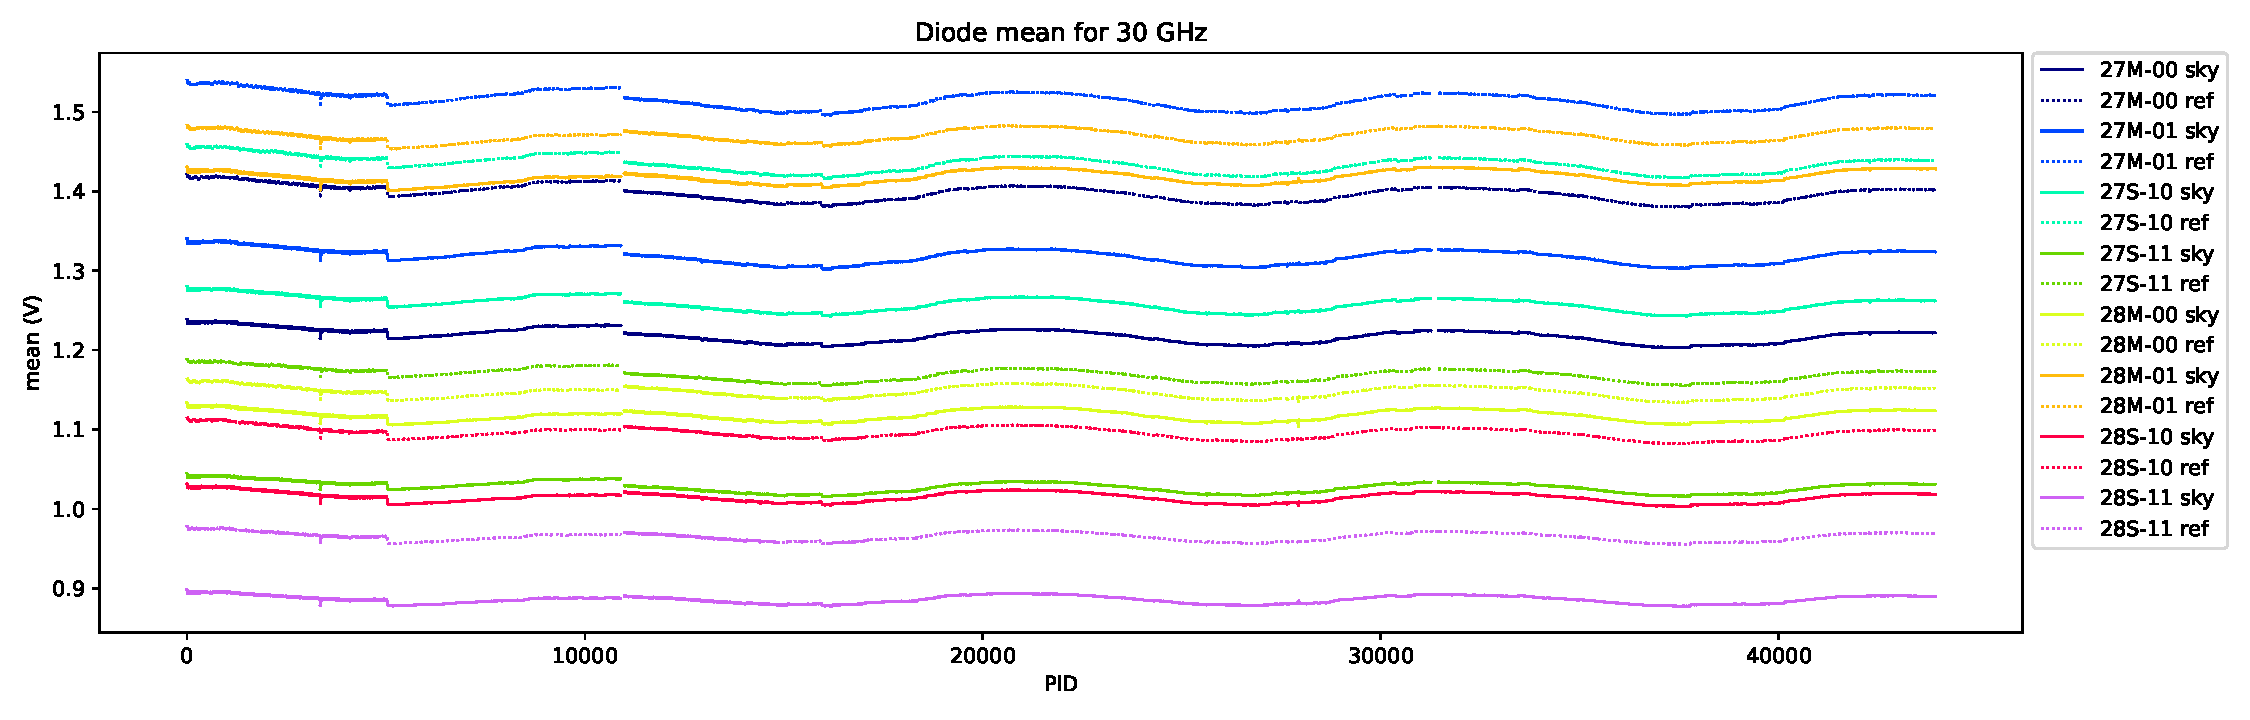
\includegraphics[width=\linewidth]{scripts/30_mean.pdf}\\
  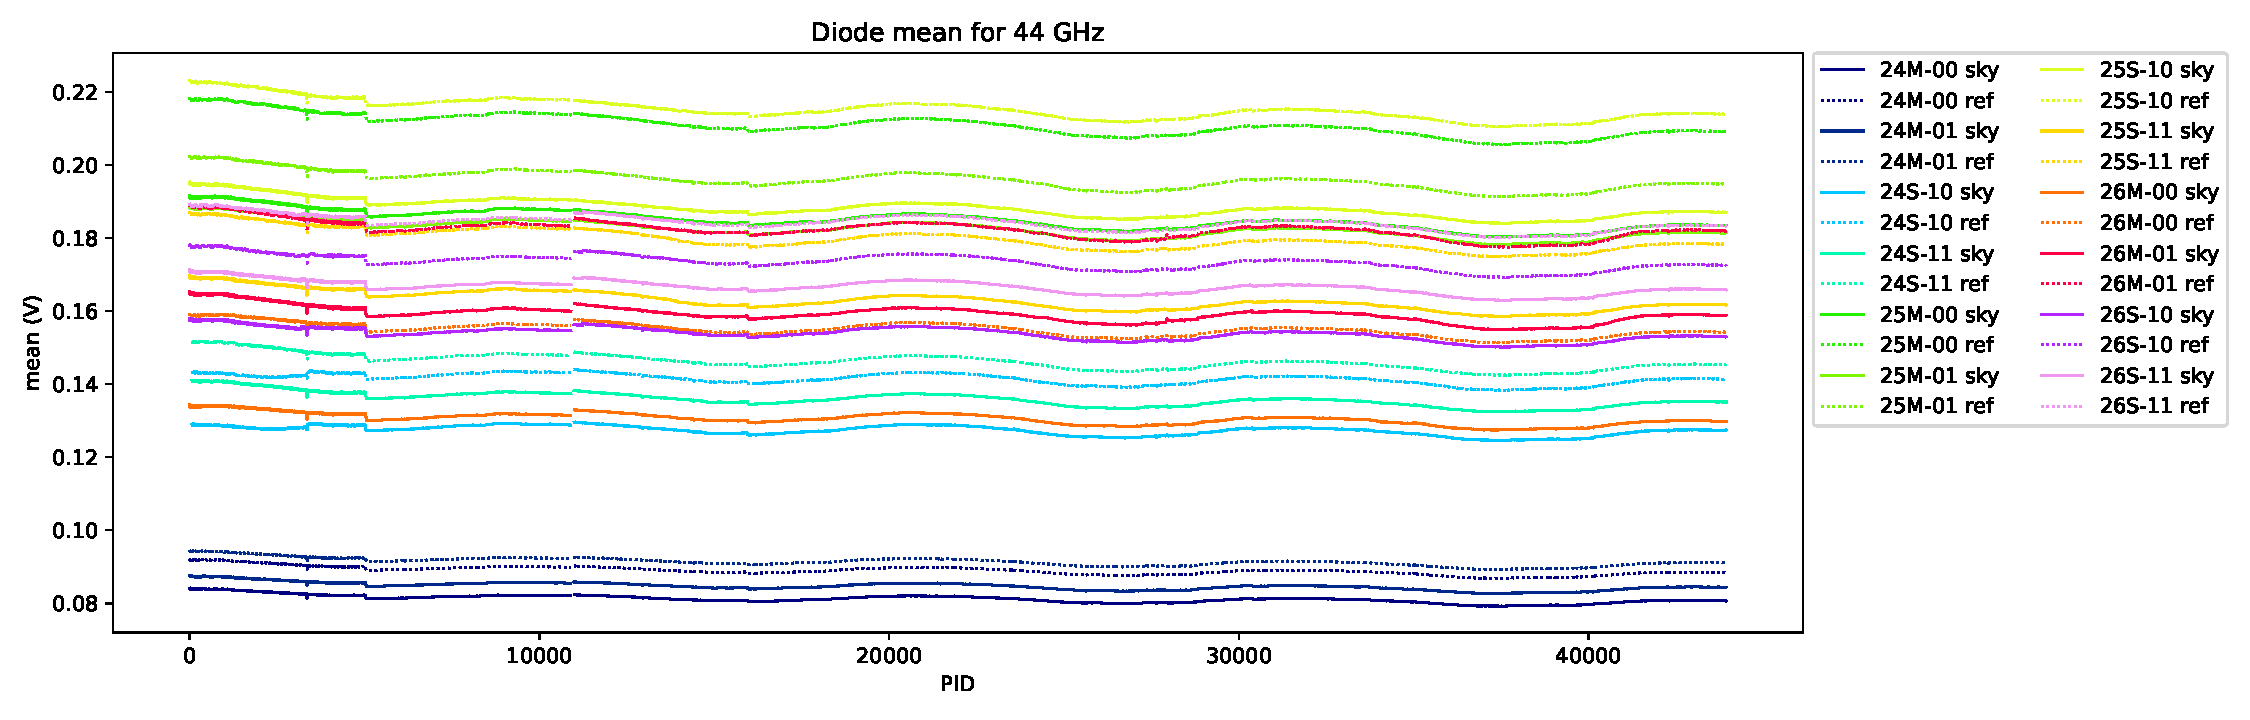
\includegraphics[width=\linewidth]{scripts/44_mean.pdf}\\
  \includegraphics[width=\linewidth]{scripts/70_mean.pdf}
  \caption{Diode means over the entire flight for (top to bottom): 30 GHz, 44 GHz and 70 GHz. 
  }\label{fig:means}
\end{figure*}

\begin{figure*}[t]
  \center
  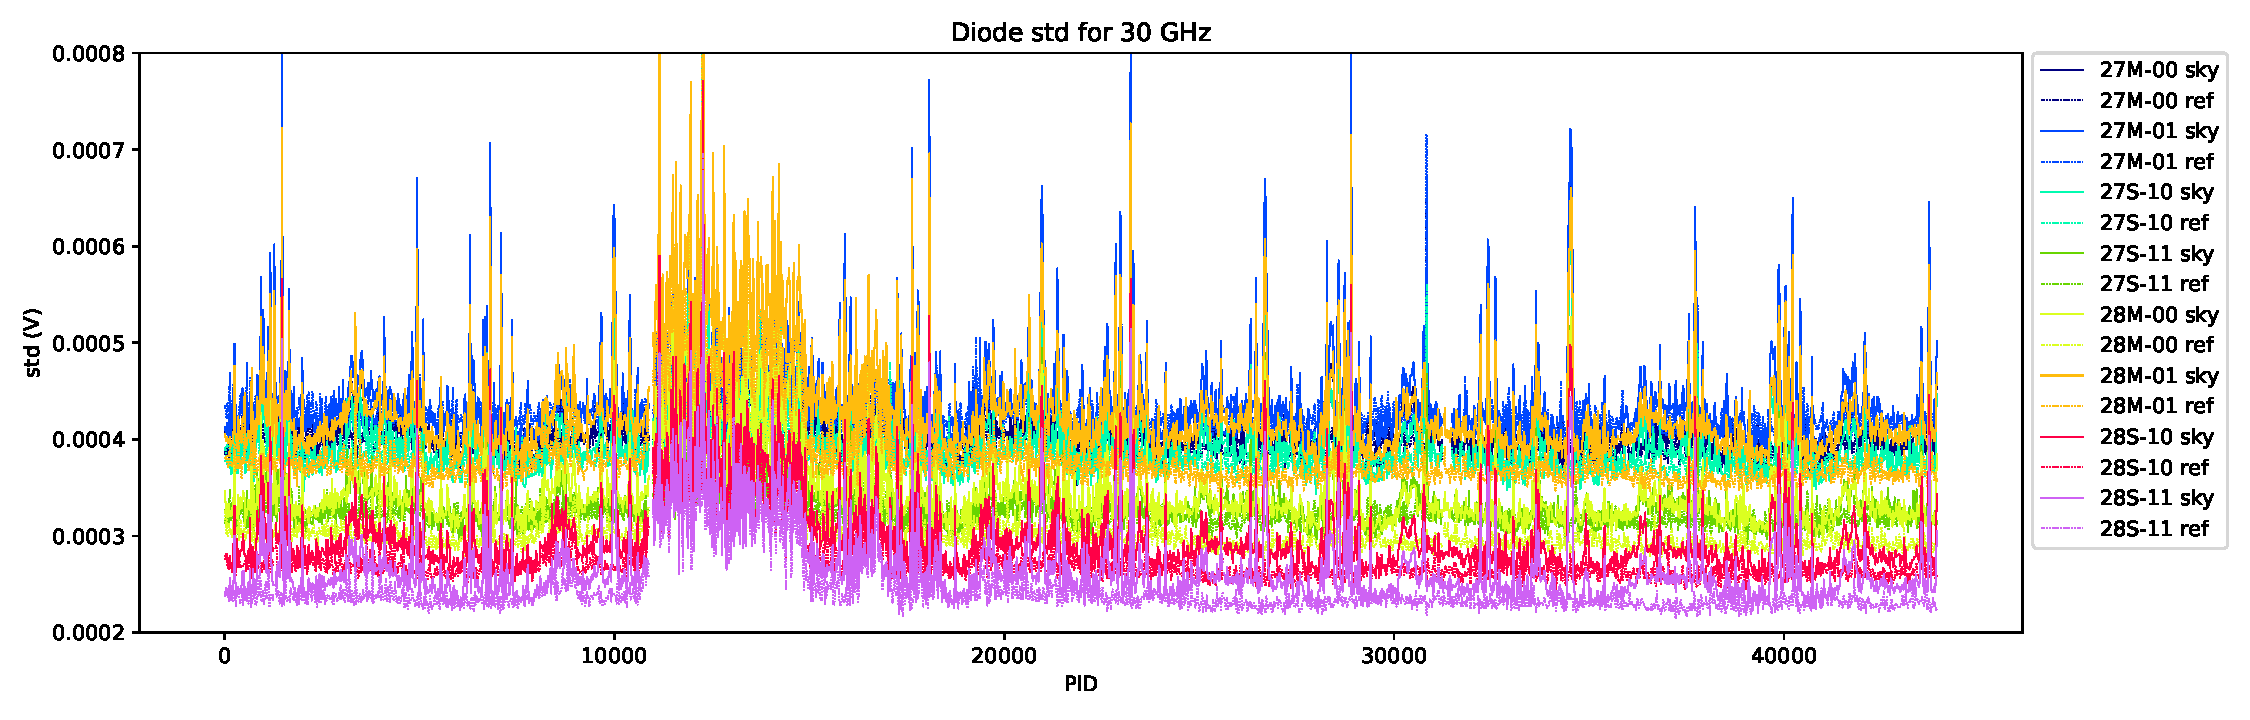
\includegraphics[width=\linewidth]{scripts/30_std.pdf}\\
  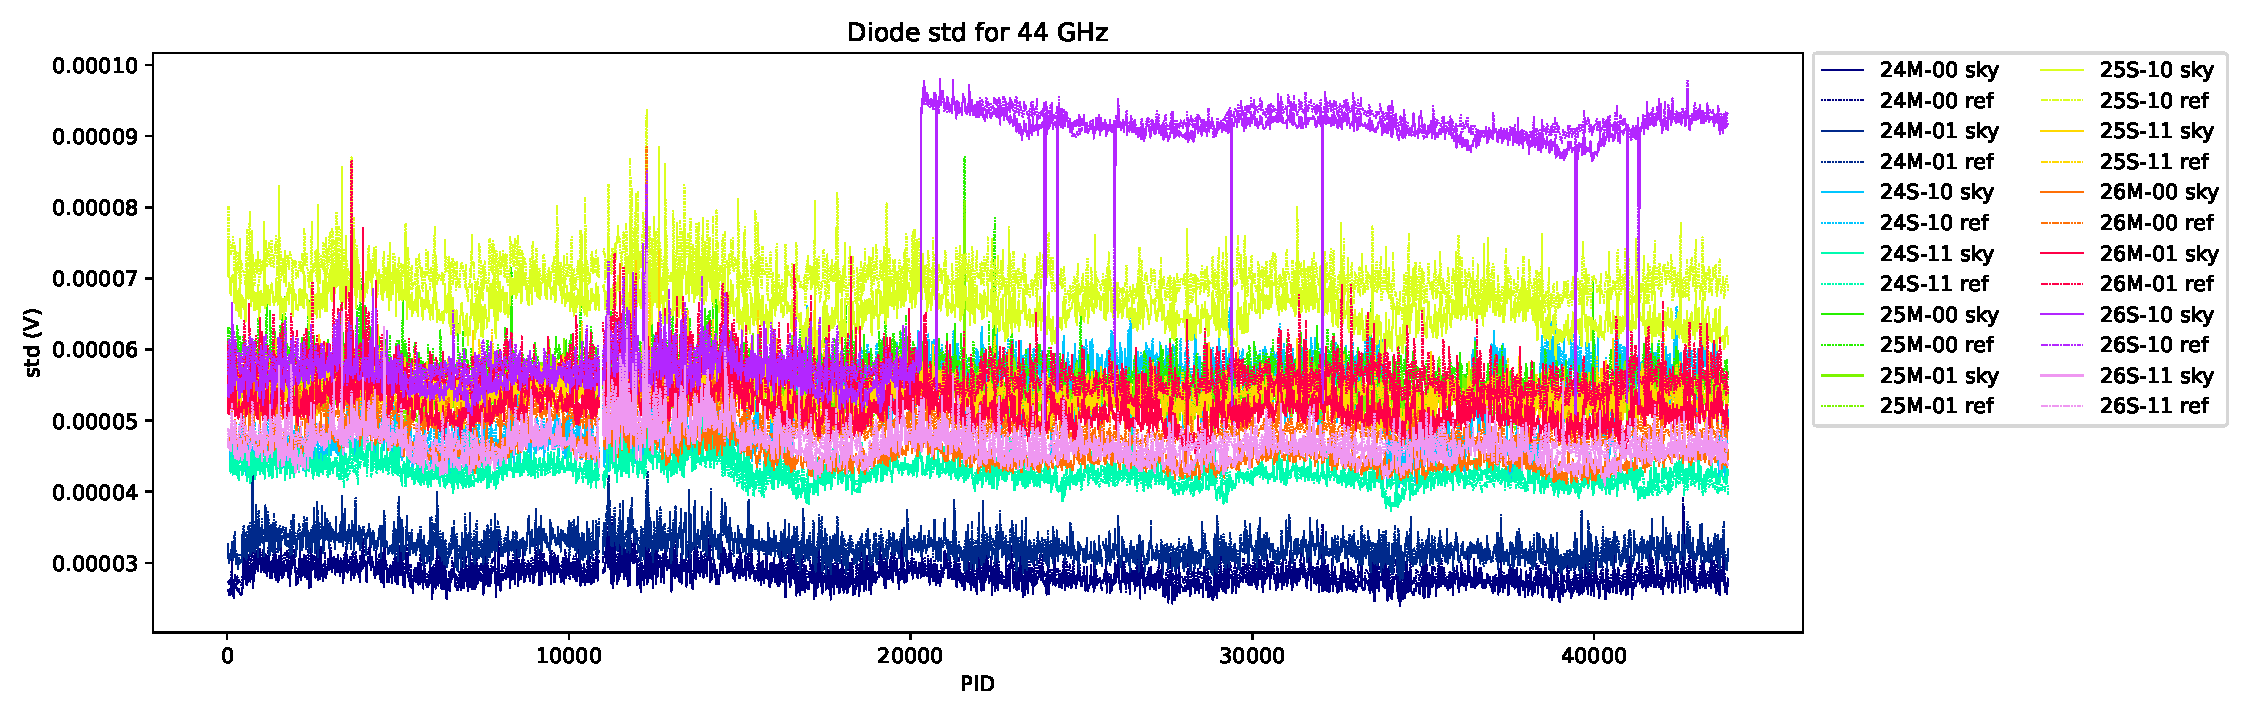
\includegraphics[width=\linewidth]{scripts/44_std.pdf}\\
  \includegraphics[width=\linewidth]{scripts/70_std.pdf}
  \caption{Diode RMS values over the entire flight for (top to bottom): 30 GHz, 44 GHz and 70 GHz. 
  }\label{fig:rms}
\end{figure*}

\begin{table}
\caption{LFI Flag Information. All flag bits not listed here are unused and can be ignored. Bolded rows indicate flags we considered for \BP\ }
\label{tab:flags}

\begin{tabular}{ c | c | c }
\hline\hline
Bit & Name & Explanation\\
\hline
4  & Maneuvers & \makecell{Planck was transitioning\\ between rings}\\
5 & Time Quality & \multirow{2}{*}{On board clock problem} \\
6 & Time Quality & \\
11 & Start/Stop Gap & Beginning or end of a gap\\
\textbf{14} & \textbf{Bad Data} & \textbf{Other data issue}\\
\textbf{16} & \textbf{Gap} & \textbf{Data is missing}\\
\textbf{18} & \textbf{Planet} & \textbf{A planet transited the beam}\\
\textbf{19} & \textbf{Moving Object} & \multirow{2}{*}{\makecell{\textbf{Another object}\\ \textbf{transited the beam}}}\\
\textbf{20} & \textbf{Moving Object} & \\
\textbf{22} & \textbf{Special Observation} & \textbf{Non-science observation}\\

\hline

\end{tabular}

\end{table}

Maybe talk about the galactic masks?

\subsection{Adc Correction}
\label{sec:adc}

Based on the work done in \citet{planck2013-p02a}, we apply a similar procedure to the LFI corrections. The tell-tale signature of non-linearities in the ADC module is a characteristic dip in the noise RMS as a function of voltage. What causes this non-linearity is not clear, but we hope to resolve this issue. As described in \citet{planck2013-p02a}, the procedure prescribed to correct for the ADC non-linearities is to solve for the deviations between the expected linear response and the observed white-noise levels as shown in (some nice figure to be provided). This method of correcting the ADC non-linearities has two potential issues that we aim to correct here. The first issue is that this method of returning the ADC response to a purely linear form removes any natural deviations in the response. Anything that is not linear is considered to be an error we need to correct. The second issue, as seen by the DPC ADC correction tables is that the corrections are only done in the high signal to noise regime. Seeing as the dips in the white noise level are consistently spaced with similar dip depths we want to correct these dips even outside the poorly sampled voltages.

Our adaptation of ADC corrections is done by creating a simple parametric model which estimates the dip width, the dip depth, and the voltage separation between dips. The dips in the white noise level are modeled as simple Gaussian functions. An example of one of this dips, with a fit Gaussian and the Gaussian corrected white noise vs voltage is shown in (another figure). We see that the Gaussian fit describes the dip well, while still allowing small scale fluctuations in the ADC white noise level. 

So how do we apply these corrections?

There are a few steps to go from modeling the dips in the white noise level to the new ADC correction tables. The modeled dips correspond to the differential response of the ADC, and we create a global differential response function by removing the linear portion of the voltage vs white noise and extrapolating the regular dips to the entire diode voltage range. What we need to correct for the ADC non-linearities is in fact the inverse differential response (I guess point to the equations from \citep{planck2013-p02a} Appendix A). This inverse differential response function, as show in (some figure) can be integrated up to return the reconstructed inverse response function (RIRF). We are almost done. In order to avoid having our corrections degenerate with the gain, we remove the linear portion of the reconstructed inverse response function. The ADC correction tables are then given by a grid of $V_{\rm in}$ and the corrected response $V_{\rm out}$, where $V_{\rm out} = V_{\rm in} + \mathrm{RIRF}$.

Then comes the future portion where we throw in some maps and show some differences between (I suppose) no ADC corrections, DPC ADC corrections, and our amazing work. Nice.

\subsection{Reference Load Smoothing}
\label{sec:refsmoothe}

Before the diodes are combined to produce the TOD, smoothing is applied to the load measurement to reduce high frequency noise, as was shown to be effective in the npipe analysis \citep{npipe}. The filter we apply is the Wiener filter, $W$, defined as 

\begin{equation}
\label{eq:wiener}
W = \frac{P_s}{P_s + P_n} = \frac{1}{1+\frac{1}{\alpha}}. 
\end{equation}

Here, $P_s$ and $P_n$ are the signal and noise powers, and $\alpha$ is the signal to noise ratio of the sky to the load. If we assume that both diode's data are Gaussian, we can estimate $\alpha$ as

\begin{equation}
\label{eq:sn}
\alpha = \frac{P_s}{P_n} = \frac{r}{1-r},
\end{equation}

where $r$ is Pearson's correlation coefficient. Inserting Eq. \ref{eq:sn} into Eq. \ref{eq:wiener} gives

\begin{equation}
W = \frac{1}{1 + \frac{1-r}{r}} = r,
\end{equation}

indicating that the Wiener filter in this case can be well approximated by the correlation coefficient between the two diodes. This is computed after the ADC corrections, as we expect this corrected timestream to have fewer artifacts. 

Figure \ref{fig:refFilters} shows the computed filters applied to each of the reference diodes as a function of frequency. Each filter follows a similar shape, serving to retain the low frequency components which will be removed from the sky in the differencing stage, while filtering the uncorrelated high frequency components. This reduces the amount of noise injected into the final TODs by the load diodes, which results in cleaner overall measurements. The filters are defined to be unity for frequencies less that $7 Hz$, which eliminates dips in the filtering functions caused by the dipole which were seen at multiples of the scan frequencies.

These filters are computed per-pid, and then averaged over the entire flight. This smoothed filter is then splined, and that spline is stored, to be applied to each chunk of the reference load data when it is processed. Contrary to our initial assumptions, there is still correlation at all scales, which is why we do not enforce the filter to be 0 at the 

\begin{figure}[t]
  \center
  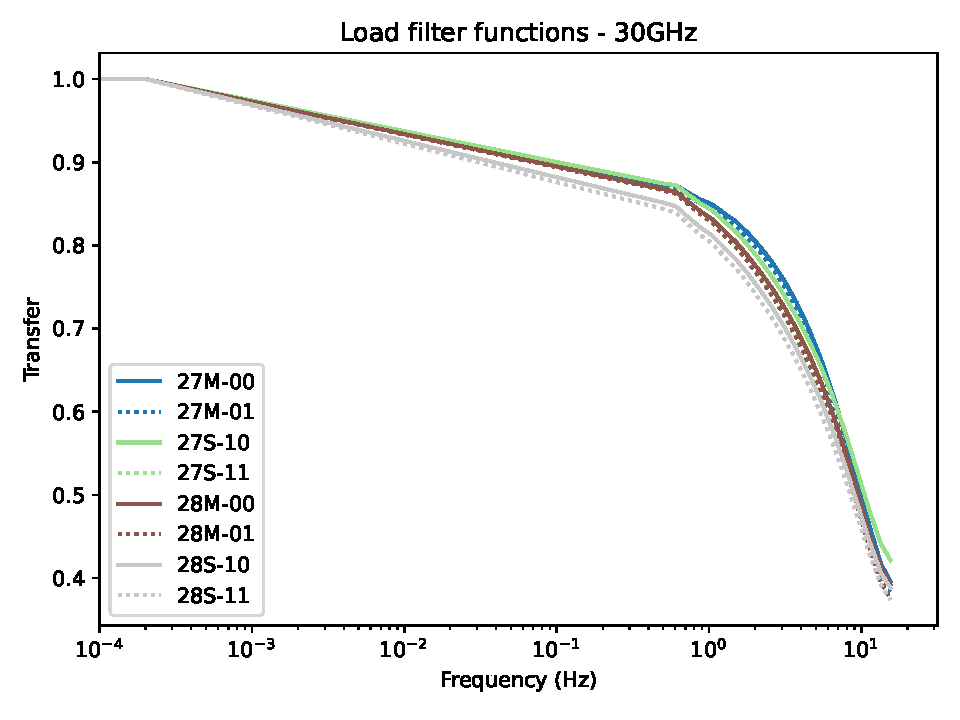
\includegraphics[width=\linewidth]{scripts/load_filters_30.pdf}\\
  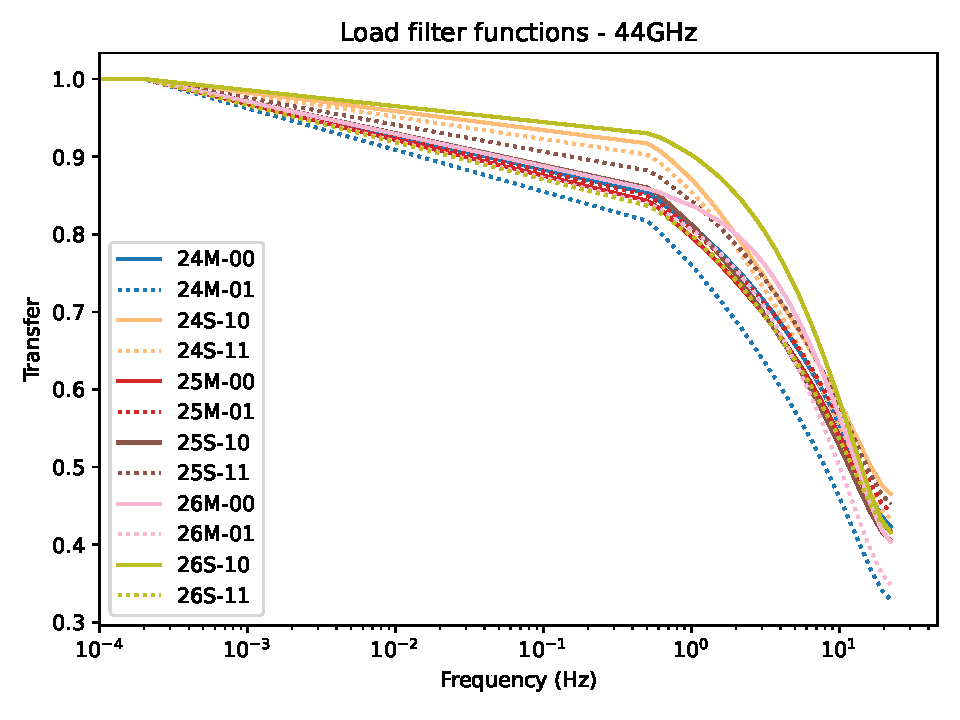
\includegraphics[width=\linewidth]{scripts/load_filters_44.pdf}\\
  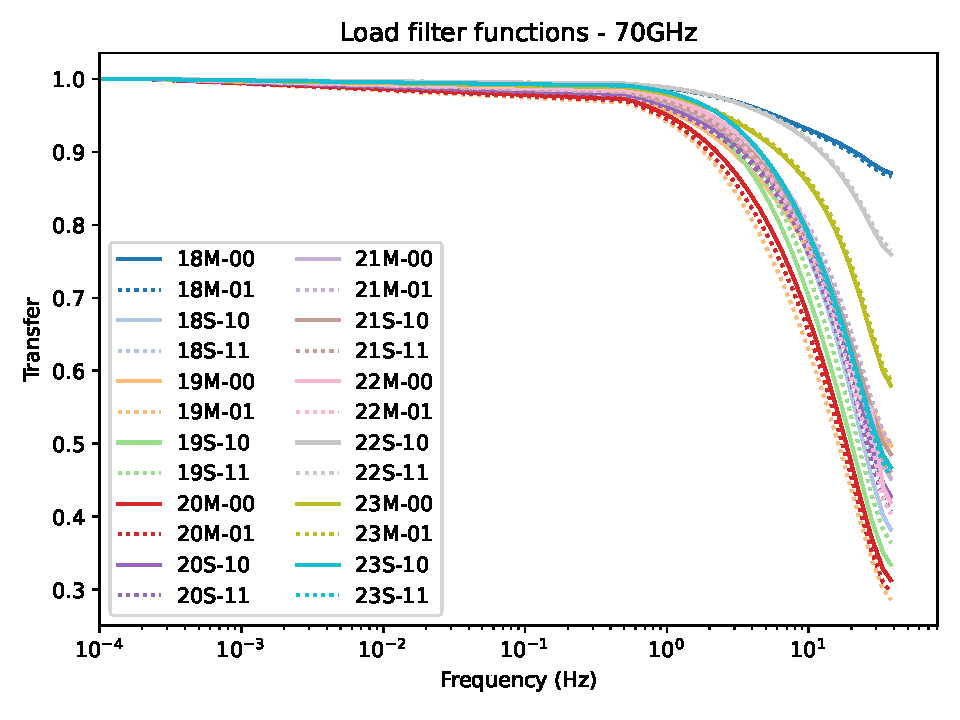
\includegraphics[width=\linewidth]{scripts/load_filters_70.pdf}
  \caption{Filter transfers as a function of frequency for (top to bottom) 30GHz, 44GHz and 70GHz LFI reference load diodes. 
  }\label{fig:refFilters}
\end{figure}



\subsection{Gain Modulation Factor}
\label{sec:gainFac}

The gain modulation factor ($r_1$ and $r_2$ in Eq. \ref{eq:datamodel}) is designed to correct the mismatch in power between the load diode, which is observing a 4K reference load, and the sky diode, which observes the 2.7K microwave sky. Historically, this value has been calculated following the procedure of  \citet{Mennella_2003}, by computing 

\begin{equation}
r = \frac{\sum^N_{i=1} V_{sky,i}}{\sum^N_{i=1} V_{ref,i}}
\end{equation}

where $N$ represents the total number of unflagged samples in each data chunk, and $V$ is the voltage data from the sky or load. This is a simple calculation that matches the average power level of the two diodes, but it is also possible to refine this simple model slightly to account for the different components of the sky signal. We can instead model the sky diode as 

\begin{equation}
d_{sky} = \alpha_1 + \alpha_2 * s_{gal} + \alpha_3 * d_{load}
\end{equation}

where $s_{gal}$ is the galactic signal and $d_{sky}$ and $d_{load}$ are the sky and load diode timestreams, respectively. This parameterization allows a simultaneous fit to the galactic signal and possible offset term, which should provide a cleaner fit to the actual noise and allow a better subtraction. The code performs a least squares minimization over each pointing period to estimate the best fit values of $\alpha$, and then uses $\alpha_3$ as the best fit value for the Gain Modulation Factor $r$.

Figure \ref{fig:GMFcompare} shows a comparison between these two estimates of the Gain Modulation Factor, as well as the published DPC values from the 2018 analysis. 

This second approach introduces a dependency on the initialization sky model, $s_{gal}$. As the L1 processing is not included in the overall Gibbs chain, due to very minimal dependencies on the rest of the chain, this sky model is not updated in future iterations and remains fixed to the initial value. Figure \ref{fig:GMFstable} shows the resulting Gain Modulation Factor for three different initial sky models, showing that this dependency is very weak. The resulting processing time reduction from not re-computing on the L1 data each iteration is therefor worth this negligible bias.

\subsection{Diode Weights}
\label{sec:weights}

Currently we just use the DPC weights. 

\section{TOD-Level Corrections}

Once the diode signals have been combined into a single TOD signal, we perform a final low level correction that was previously computed at the diode level. The 1Hz spike template has been moved to the TOD level in our analysis, simplifying the process and number of templates that must be computed, without loss of accuracy. This is possible because the combined TOD is linear in the diode data, so a 1Hz template can be computed that is effectively the combination of the four diode-level templates computed in previous analyses. 


\subsection{1 Hz Spike Templates}
\label{sec:1Hz}

\section{Propagation of Errors}
\label{sec:uncertainties}

Here we compare two pipeline runs, one with the low level parameters sampled and one with them fixed. We show that the effects of the uncertainties of the low lever parameters are small compared to other uncertainties, and thus we are justified in fixing them.

\section{Comparison with DPC}
\label{sec:comparison}

We can compare the final TOD generated using the \BP\ pipeline to the L2 data used in the DPC analysis to see what effects these procedures have had.

\section{Conclusions}
\label{sec:conclusions}

The \BP\ pipeline has successfully reproduced and improved the Planck DPC low level processing, incorporating improvements from the npipe analysis as well as novel ideas. The resulting TOD is available to the rest of the pipeline, and they have cleaner noise properties than the existing DPC timestreams. 

\begin{acknowledgements}
  We thank Prof.\ Pedro Ferreira and Dr.\ Charles Lawrence for useful suggestions, comments and 
  discussions. We also thank the entire \Planck\ and \WMAP\ teams for
  invaluable support and discussions, and for their dedicated efforts
  through several decades without which this work would not be
  possible. The current work has received funding from the European
  Union’s Horizon 2020 research and innovation programme under grant
  agreement numbers 776282 (COMPET-4; \BP), 772253 (ERC;
  \textsc{bits2cosmology}), and 819478 (ERC; \textsc{Cosmoglobe}). In
  addition, the collaboration acknowledges support from ESA; ASI and
  INAF (Italy); NASA and DoE (USA); Tekes, Academy of Finland (grant
   no.\ 295113), CSC, and Magnus Ehrnrooth foundation (Finland); RCN
  (Norway; grant nos.\ 263011, 274990); and PRACE (EU).
\end{acknowledgements}


\bibliographystyle{aa}

\bibliography{sources.bib,../common/Planck_bib,../common/BP_bibliography}


\end{document}
